\section{The model}
\label{sec:dsmc_model}
The Direct Simulation Monte Carlo (DSMC) can be seen as either a simplified, stochastic Molecular Dynamics algorithm, or a Monte Carlo method for solving the time-dependent nonlinear Boltzmann equation. The physical system consists of $N$ atoms in a box with volume $V$ and porosity $\phi$, where only the volume $V' = \phi V$ is available for atoms. This is illustrated in figure \ref{fig:cylinder}.
\begin{figure}[h]
\begin{center}
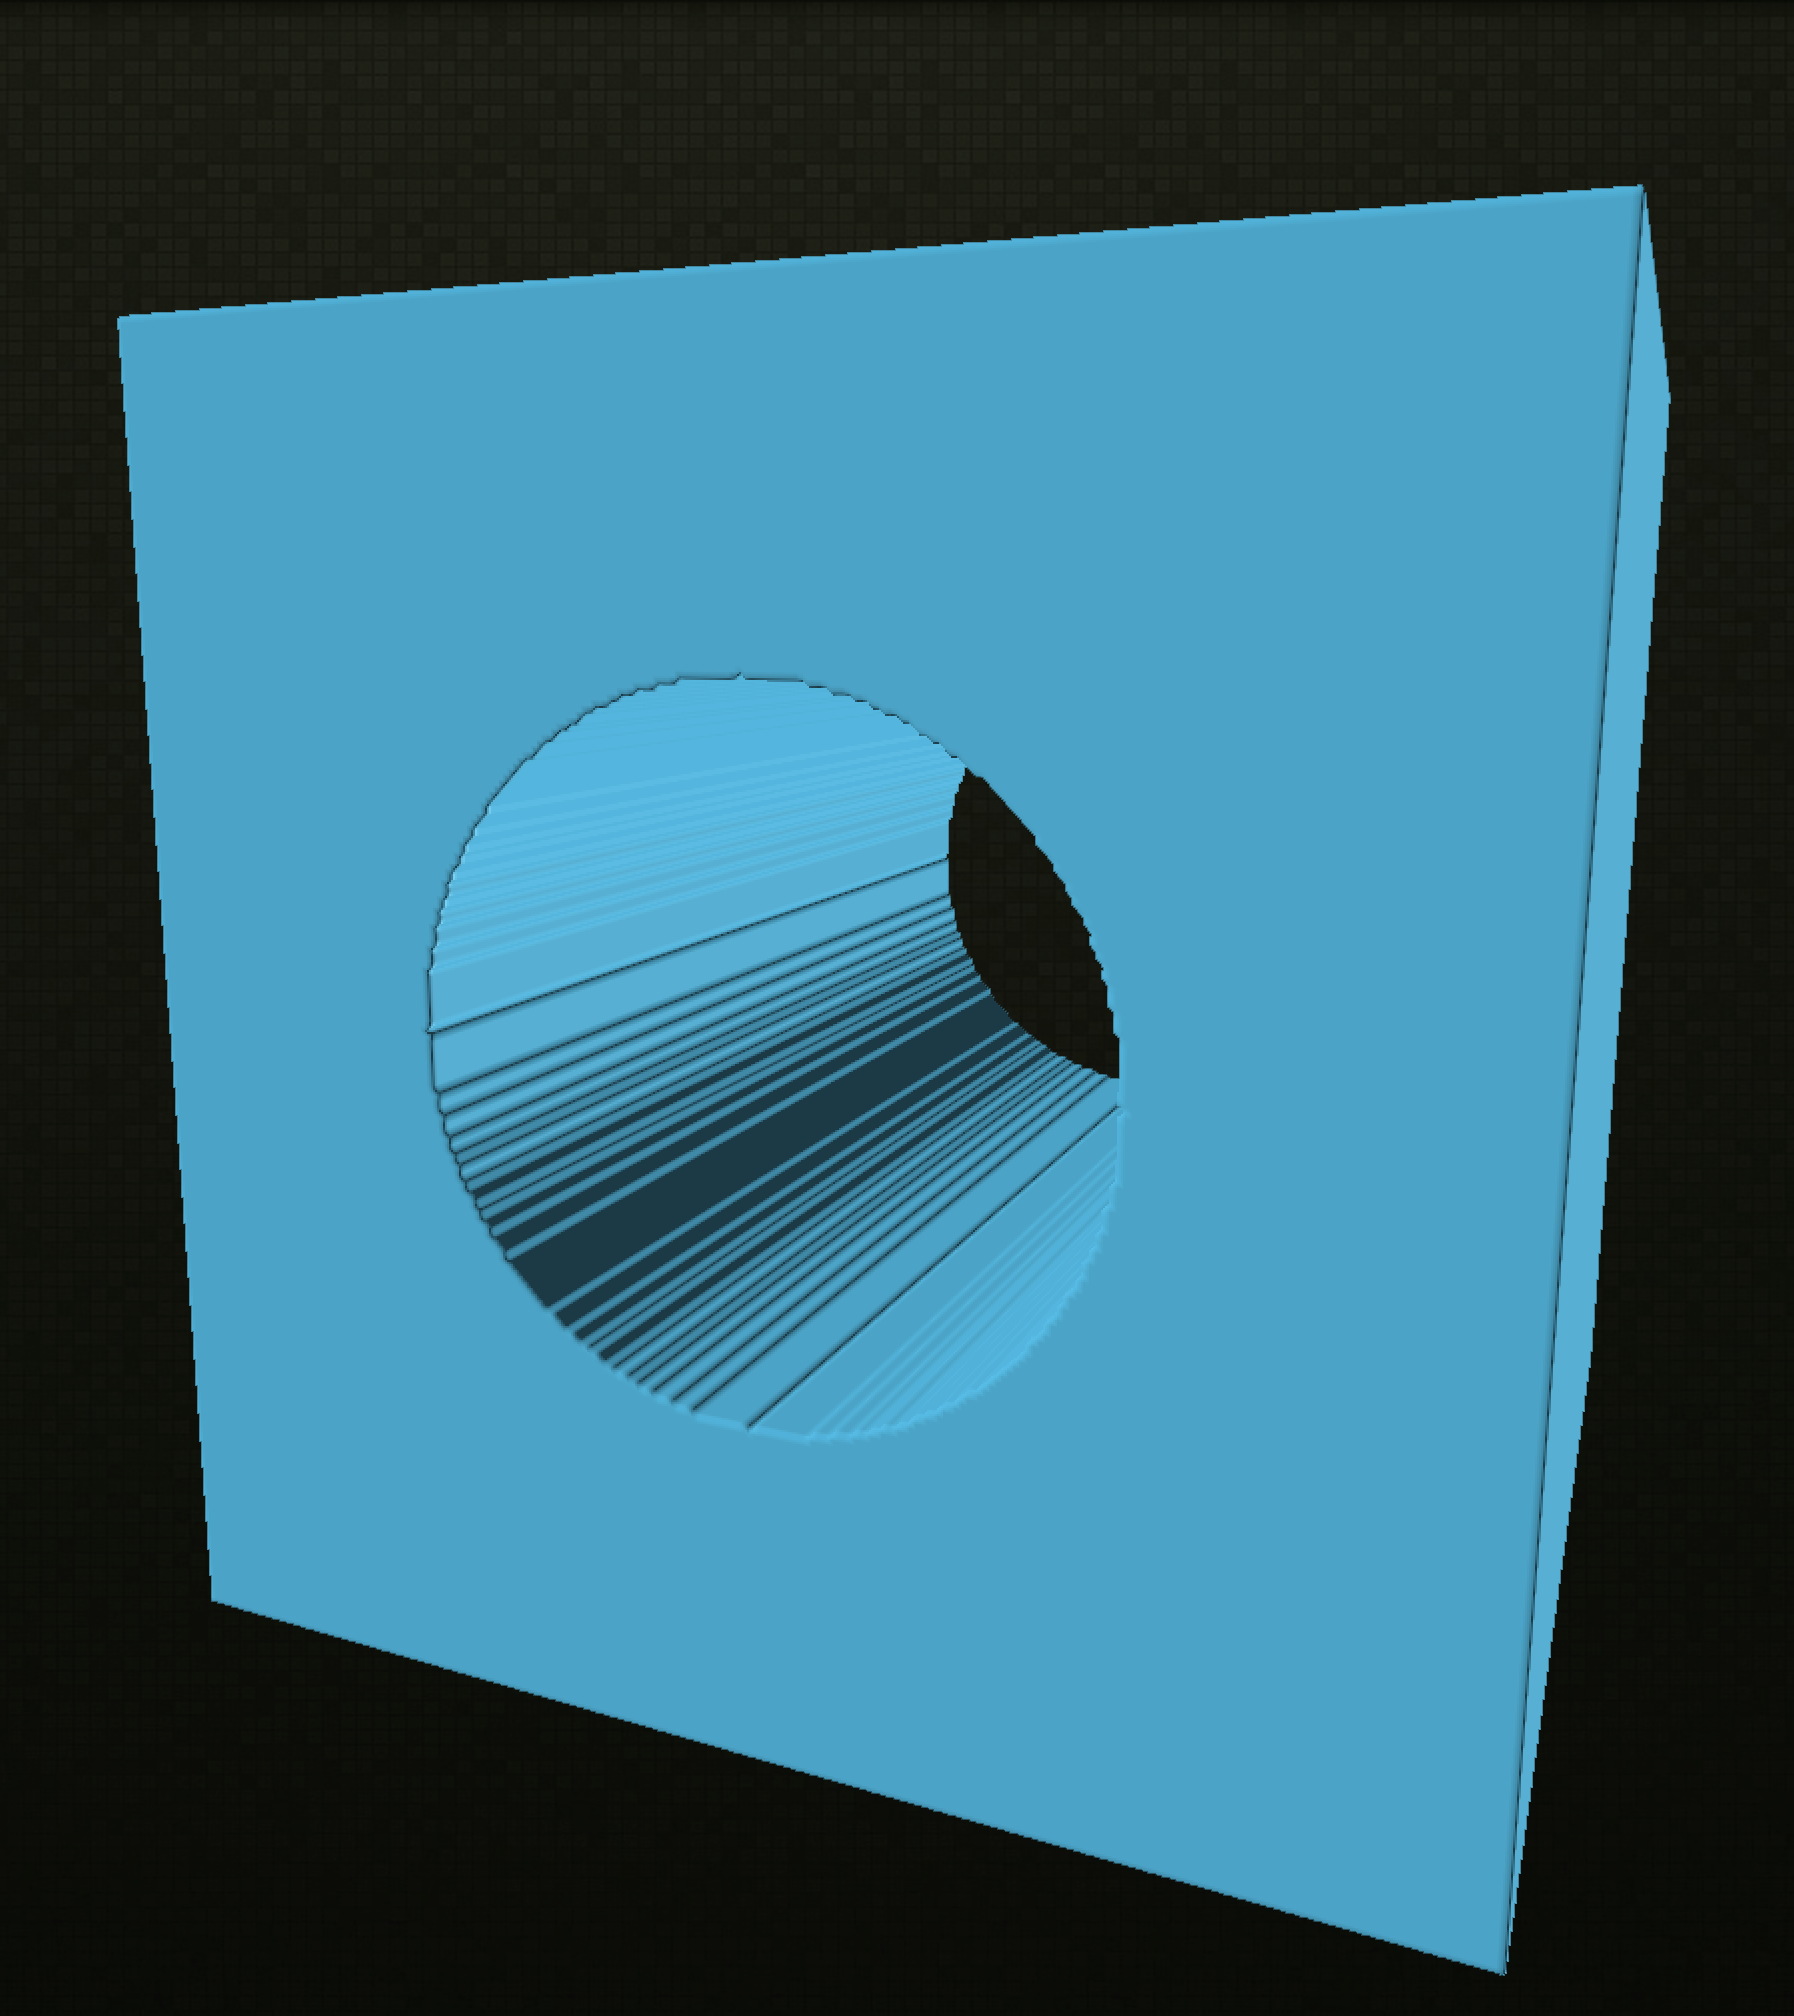
\includegraphics[width=\textwidth, trim=0cm 0cm 0cm 0cm, clip]{DSMC/figures/cylinder.png}
\label{fig:cylinder}
\end{center}
\caption{Example of a system with volume $V$ and total available volume $V' = \phi V$.}
\end{figure}
Instead of tracking the trajectory of each atom, we simulate $M$ particles, each representing $N_{eff}$ real atoms. We can interpret this approximation as the assumption that all atoms in a small region of space around a simulated particle move with approximately with the same velocity. The state of a DSMC simulation is, as in MD, fully described by $6M$ phase variables, three velocities and three positions per simulated particle. Since we don't have detailed information about the positions of all the real atoms, we cannot calculate forces as is done in MD. Instead, we use the assumtion that the gas particles only experience binary collisions (all three-particle interactions are negligible), just like we did while deriving the Boltzmann equation in section \ref{sec:boltzmann_equation}. Collisions are performed in a stochastic manner, where the rate of collisions and post-collision velocities are determined from kinetic theory. This collision operator can bee viewed as a stochastic function $\mathcal{C}(\vec q, \vec p, \mathcal{G})$, where $\vec q$ and $\vec p$ form the phase space point and $\mathcal G$ contains all information about the system geometry.\\
The equation of motion is integrated by applying the standard Euler method on the positions so that $\vec r_i(t+\Delta t) = \vec r_i(t) + \vec v_i(t)\Delta t$ for all particles. If a particle interacts with a boundary during the timestep, some sort of surface interaction rule is applied before the timestep is continued (note that a particle may collide with the surface several times during a single timestep). The particle movement can be seen as another stochastic operator $\mathcal{M}(\vec q, \vec p, \mathcal{G})$. Different surface interaction models are discussed in section \ref{sec:surface_interactions}. After all particles are moved, a number of particles are chosen to undergo binary collisions. The details of this collision rule is discussed in the next subsection.\\
A crucual detail worth mentioning is that we have splitted the timestep into two parts; moving and colliding. This is a reasonable assumption as long as the timestep $\Delta t$ is smaller than the mean collision time $\tau_{coll}$
\begin{align}
	\Delta t \leq \tau_{coll} = {1\over \sqrt 2 \pi \sigma^2 \rho_n \langle v \rangle}.
\end{align}
Statistical properties are sampled at the end of each timestep where most physical quantities are sampled as time averages. A flow chart illustrating the steps of a typical DSMC algorithm is presented in figure \ref{fig:dsmc_flowchart}.
\begin{figure}[h]
\begin{center}
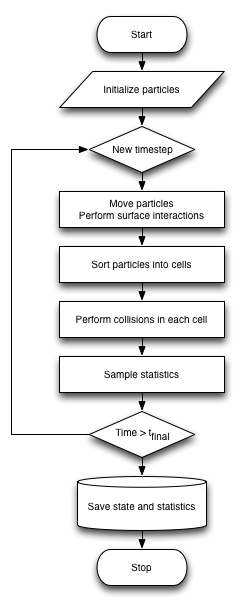
\includegraphics[width=0.5\textwidth, trim=0cm 0cm 0cm 0cm, clip]{DSMC/figures/dsmc_flowchart.png}
\label{fig:dsmc_flowchart}
\end{center}
\caption{Typical steps for a DSMC algorithm.}
\end{figure}

\subsection{Collisions}
In an MD simulation it is not clear how one would define a \textit{collision event} since the atoms interact through a continuous force field. If two equal atoms with the same velocity move towards each other, the atoms would at some point reverse their velocity. In this case, one could define the collision event to occur at the time when their relative distance is at its minimum, but other equally valid definitions could be argued for. However, it is clear that a collision should be identified as an event that happens when the atoms are close, i.e. short ranged forces. In this thesis, we have implemented the \textit{hard sphere} model, in which each particle is assumed to be a perfect hard sphere with diameter $d$ and mass $m$. Generally, two particles with radius $R_1$ and $R_2$ will undergo an elastic collision if their displacement is equal to the sum of their radii. In DSMC, we will apply a stochastic hard sphere collision model.\\
\subsubsection{Number of collisions}
We choose the collision pairs at random, and to ensure that only nearby particles collide, the particles are sorted into spatial cells whose volumes are typically smaller than a cubic mean free path. If we select two particles $i$ and $j$ with relative velocity $\vec v_r$ and cross section $\sigma=\pi d^2$, each representing $N_{eff}$ real atoms in a cell with volume $V_c$, the total volume sweeped out during a timestep is
\begin{align}
	V_{sweep} = N_{eff}\sigma^2|\vec v_r|\Delta t.
\end{align}
The probability of collision is the total sweeped volume $V_{sweep}$ divided by the total cell volume $V_c$
\begin{align}
	P = {N_{eff}\sigma^2|\vec v_r|\Delta t \over V_c},
\end{align}
so by choosing $N(N-1)/2$ such pairs, the number of collisions $M_{coll}$ will be
\begin{align}
	M_{coll} = {N(N-1)N_{eff}\sigma^2\langle v_r \rangle \Delta t\over 2 V_c},
\end{align}
where we replaced the relative velocity $v_r$ by the mean value in the cell
\begin{align}
	\langle v_r \rangle = {1\over N} \sum_{i,j} |\vec v_i - \vec v_j|.
\end{align}
Instead of calculating the mean relative velocity in each cell every timestep, we instead calculate $M_{cand}$ collision \textit{candidate pairs} so that
\begin{align}
	{M_{coll}\over M_{cand}} = {\langle v_r\rangle \over v_r^{max}},
\end{align}
since the probability of collision is proportional to the relative velocity. Each of these candidates go through an acceptance-rejection process where we pick a uniform random number $\mathcal{R}_1\in (0,1)$ and accept the collision if
\begin{align}
	v_r \leq v_r^{max}\mathcal{R}_1.
\end{align}
This will only accept $\langle v_r\rangle/v_r^{max}$ of the candidates and we end up with $M_{coll}$ actual collisions, as desired. Note that even particles that move away from each other can collide. This property has, as we will see in section \ref{sec:dsmc_eos}, an interesting consequence leading to which equation of state the gas satisfies.
\subsubsection{Post-collision velocities}
After a particle pair collision is accepted, we want to select new velocities conserving both energy and momentum. We need a total of six equations to determine the post-collision velocities where four are provided through the conservation laws. Conservation of momentum yields that the center of mass velocity is unchanged
\begin{align}
	\vec v_{cm} = \frac{1}{2}(\vec v_i + \vec v_j) = \frac{1}{2}(\vec v_i^* + \vec v_j^*) = \vec v_{cm}^*,
\end{align}
where the energy conservation tells us that the relative velocity vector does not change its magnitude
\begin{align}
	v_r = |\vec v_i - \vec v_j| = |\vec v_i^* - \vec v_j^*| = v_r^*.
\end{align}
The two remaining degrees of freedom are determined by choosing the direction of the relative velocity
\begin{align}
	\vec v_r^* = v_r\left[(\sin\theta\cos\phi)\vec i + (\sin\theta\sin\phi) \vec j + (\cos\theta)\vec k\right],
\end{align}
where the angles are uniformly distributed over the unit sphere. The area element $d\Omega$ can be written as
\begin{align}
	d\Omega = \sin\theta d\theta d\phi = -d\phi d(\cos\theta),
\end{align}
so we need to choose $\phi$ and $\cos\theta$ uniformly. This is easy, we simply choose 
\begin{align*}
	\phi = 2\pi\mathcal{R}_2 & \qquad \qquad \cos\theta = 2\mathcal{R}_3 - 1,
\end{align*}
where we calculate $\sin\theta = \sqrt{1 - \cos^2\theta}$. The post-collisions velocities are then found by
\begin{align}
	\vec v_i^* = \vec v_{cm} + \frac{1}{2}\vec v_r^*\\
	\vec v_j^* = \vec v_{cm} - \frac{1}{2}\vec v_r^*.
\end{align}
An example of how this can be implemented is found in listing \ref{lst:post_collisions_velocities}.
\begin{lstlisting}[caption=Determining post-collision velocities., label=lst:post_collisions_velocities]
void collide_molecules(Vector3 &v0, Vector3 &v1, Random *rnd) {
	Vector3 v_center_of_mass = 0.5*(v0 + v1);
	double relative_velocity_magnitude = (v1 - v2).length();
    
    double cos_theta = 1.0 - 2.0*rnd->next_double();
    double sin_theta = sqrt(1.0 - cos_th*cos_th);
    double phi = 2*M_PI*rnd->next_double();

    Vector3 relative_velocity(1,1,1)*relative_velocity_magnitude;
    relative_velocity.x *= cos_theta;
    relative_velocity.y *= sin_theta*cos(phi);
    relative_velocity.z *= sin_theta*sin(phi);
    v0 = v_center_of_mass + 0.5*relative_velocity;
    v1 = v_center_of_mass - 0.5*relative_velocity;
}
\end{lstlisting}
